\section{Case Study}\label{sec:casestudy}

To demonstrate the utility of our modular parsing approach, we
implemented parsers for the first 18 calculi~\footnote{There are some more calculi in the book,
  but they are either not ported by the implementation we compare with, or just repeats the syntax of former ones.}
from the \textit{Types and Programming Languages} (TAPL)
\cite{pierce2002types} book.
We compared our implementation with a non-modular implementation
available online, which is also written in Scala and uses the same Packrat parsing library.
We counted source lines of code (SLOC) and measured execution time for both implementations.
The result suggests that our implementation saves 69\% code comparing
with that non-modular one, but there is a 43\% slowdown due to code modularity.

\subsection{Implementation}\label{subsec:implementation}

TAPL introduces several calculi from simple to complex, by gradually adding new features to syntax.
These calculi are suitable for our case study for mainly two reasons. Firstly, they capture many of the language features
required in realistic programming languages, such as lambdas, records and polymorphism.
Secondly, the evolution of calculi in the book reveals the advantages of modular representation
of abstract syntax and modular parsing, which is the key functionality
of our approach. By extracting common components from those calculi
and reusing them, we obtain considerably code reuse as shown later.

%% \paragraph{Extracting Language Components}
We extract reusable components from all the calculi using the pattern
demonstrated in Section~\ref{subsec:language-component}. Each
component, which may contain several syntactical structures,
represents a certain feature. They are combined together as needed to
build a calculus. For example, the calculus \lstinline{Untyped} in our case study,
representing the famous untyped lambda calculus, consists of component
\lstinline{VarApp} (for variables and applications)
and component \lstinline{UntypedAbs} (for untyped lambdas).

%% For example, the \lstinline{VarApp} component below represents variables and
%% function applications.

%% \lstinputlisting[linerange=13-29]{code/src/papercode/Sec6CaseStudy/Code1.scala}% APPLY:linerange=CASESTUDY_VARAPP

Figure \ref{fig:dependency} shows the
dependency of all the components and calculi in our case study. Grey
boxes are calculi and white boxes are components. An arrow starting
from box A to box B denotes that B includes and thus reuses A.

\begin{figure*}
    \centering
    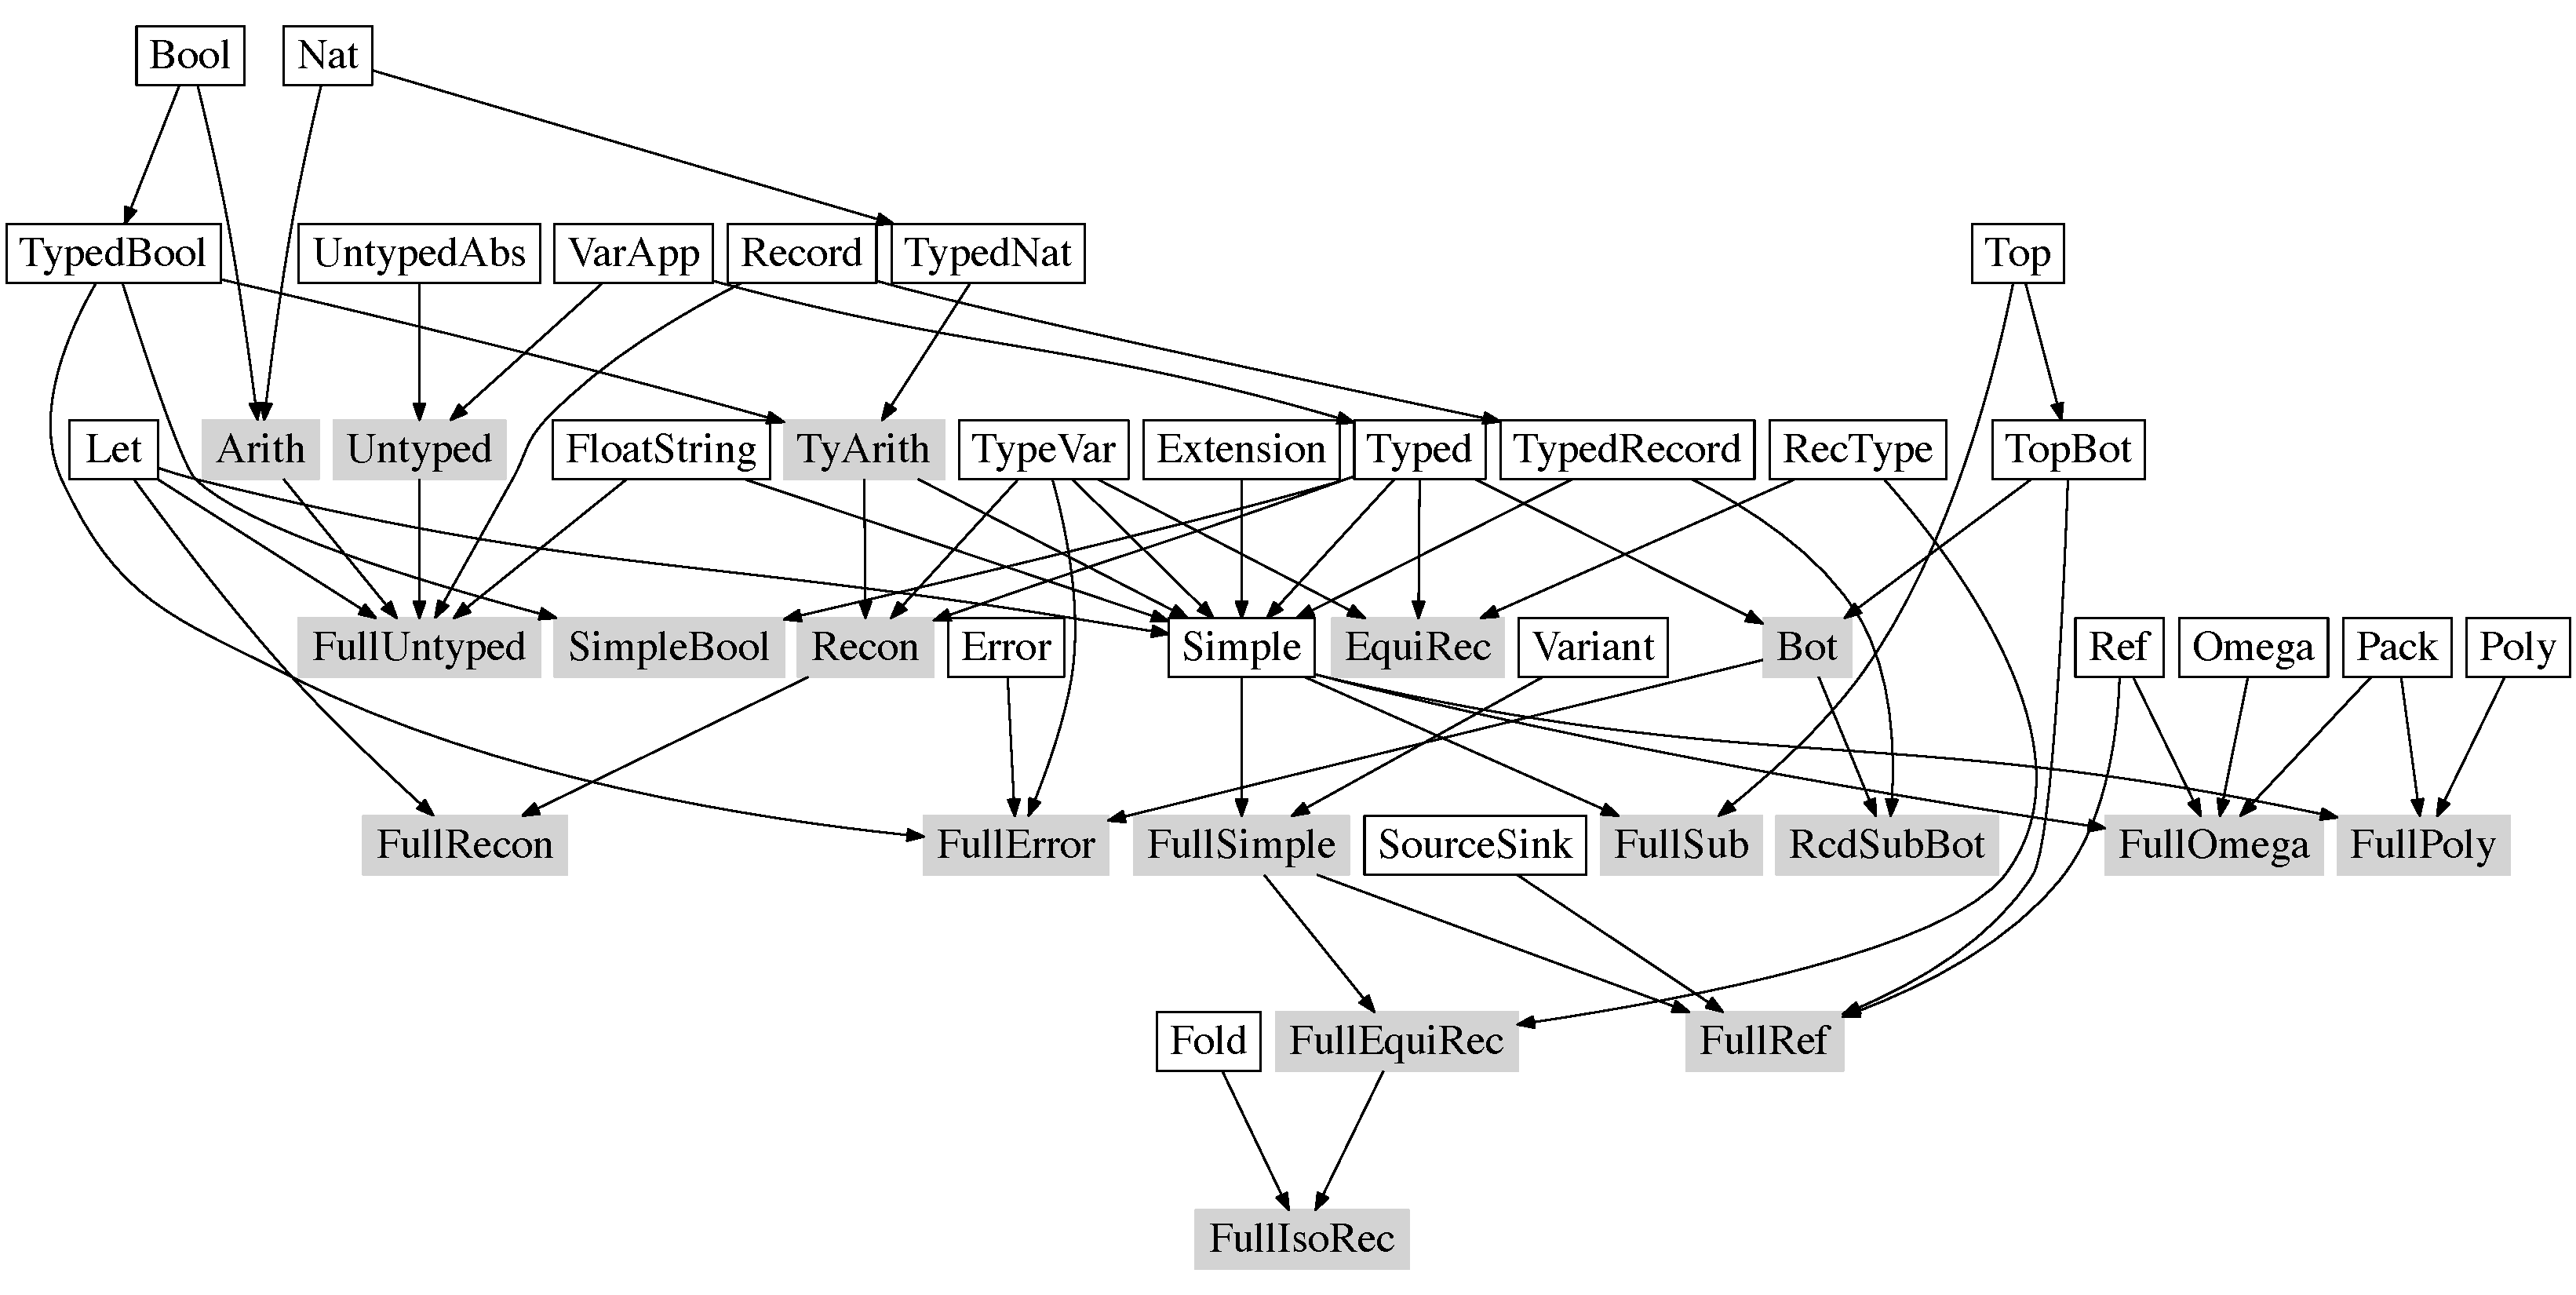
\includegraphics[width=0.8\textwidth]{resources/depGraph.pdf}
    \caption{Dependency graph of all calculi and components. Grey boxes are calculi; white boxes are components.}
    \label{fig:dependency}
\end{figure*}

Each component or language is represented by a Scala object which includes \lstinline{Alg}
for the abstract syntax, \lstinline{Print} for pretty-printing, and \lstinline{Parse} for parsing.
Since calculi and components have similar signatures, each calculus
can also be extended and reused directly. For example, calculus \lstinline{FullRef} extends from
calculus \lstinline{FullSimple}.

%% We have some naming conventions in our code, \lstinline{E} represents
%% expressions, \lstinline{T} represents types and \lstinline{K}
%% represents kinds. They are the three sorts of syntax in our case study.
%% In the component \lstinline{VarApp} we only have expressions. We use some helper traits for eliminating duplicate definitions, such as \inlinecode{EParser} containing \inlinecode{pE} for parsing expressions.

%% \lstinputlisting[linerange=9-9]{code/src/papercode/Sec6CaseStudy/Code1.scala}% APPLY:linerange=CASESTUDY_EPARSER

%% \paragraph{Composing Language Components}


%% The code of building \lstinline{Untyped} is presented in Figure~\ref{fig:casestudy-untyped}. Note that in the parser \inlinecode{Parse}, we need to override the object algebra interface and
%% parsing functions accordingly.

%% \begin{figure}[t]
%% \lstinputlisting[linerange=33-60]{code/src/papercode/Sec6CaseStudy/Code1.scala}% APPLY:linerange=CASESTUDY_UNTYPED
%% \caption{Build the \inlinecode{Untyped} calculus by composing to language components.}\label{fig:casestudy-untyped}
%% \end{figure}


%% \paragraph{Dependency Overview}

%% As shown in the graph, some components such as \lstinline{VarApp} are
%% created from scratch, while others such as \lstinline{Typed} are
%% extended from existing components.

%% From the graph, we know that common components such as \lstinline{VarApp} are reused in
%% lots of calculi. Such reuse could shorten the code considerably.
%% Next subsection examines amount of code as well as performance.

\subsection{Comparison}\label{subsec:cs-comparison}

\newcommand\ourimpl{$\texttt{Mod}_{\texttt{OA}}$}
\newcommand\ilyaimpl{\texttt{NonMod}}
\newcommand\ourclass{$\texttt{Mod}_{\texttt{CLASS}}$}
\newcommand\ilyalongest{$\texttt{NonMod}_{\texttt{|||}}$}

We compared our implementation (named \ourimpl{}) with an implementation
available online\footnote{https://github.com/ilya-klyuchnikov/tapl-scala/} (named \ilyaimpl{}).
\ilyaimpl{} is suitable for comparison, because it is also
written in Scala using the same parser combinator library.
\ilyaimpl{} implements parsers 18 calculi in TAPL in a non-modular
way. Thus \ilyaimpl{} is not able to reuse existing
code when those calculi share common features.
\ourimpl{} implements the same 18 calculi, but reuse 
is possible due to modularity.

The comparison is made from two aspects. First, we want to discover
the amount of code reuse using our modular parsing approach.
For this purpose, we measured source lines of code (SLOC) of two implementations.
Second, we are interested to assess the performance penalty caused by modularity.
Thus we compared the execution time of parsing random expressions between two implementations.

\paragraph{Standard of Comparison}
In the SLOC comparison, all blank lines and comments are excluded,
and we formatted the code of both implementations to guarantee that
the length of each line does not exceed 120 characters. Furthermore,
because \ilyaimpl{} has extra code such as semantics,
we removed all irrelevant code and only keep abstract
syntax definition, parser and pretty-printer for each calculus, to
ensure a fair comparison.

For the comparison of execution time, we built a generator to randomly
generate valid expressions for each calculus, according to its syntax. These expressions are
written to test files, one file per calculus. Each test file consists of 500
expressions randomly generated, and the size of test files varies from 20KB to 100KB.
We run the corresponding parser to parse the file and the pretty-printer to print the result.
The average execution time of 5 runs excluding reading input file was calculated, in milliseconds.

\begin{table*}
    \centering
    \resizebox{0.7\textheight}{!}{
    \begin{tabular}{|l|r|r|r|r|r|r|r|r|r|r|}
      \hline
        \multirow{2}{*}{\bfseries Calculus Name} & \multicolumn{3}{ c| }{\bfseries SLOC} & \multicolumn{7}{ c| }{\bfseries Time (ms)} \\ \cline{2-11}
        \multicolumn{1}{|c|}{} & \ilyaimpl{} & \ourimpl{} & \bfseries (+/-)\% & \ilyaimpl{} & \ourimpl{} & \bfseries (+/-)\% & \ilyalongest{} & \bfseries (+/-)\% & \ourclass{} & \bfseries (+/-)\% \\
      \hline
      \begin{tabular}{|c|c|c|}
  \hline
  t1 & t2 & t3 \\
  y1 & val1 & val4 \\
  y2 & val2 & val3 \\
  \hline
\end{tabular}

      \hline
      \multicolumn{7}{c}{}
    \end{tabular}}
    \caption{Comparison of SLOC and execution time.}
    \label{tab:comparison}
    \vspace{-0.3cm}
\end{table*}

\paragraph{Comparison Results}
Table \ref{tab:comparison} shows results of the comparison.
Let us only check \ourimpl{} and \ilyaimpl{} for now.
The overall result is that 69.2\% of code is reduced using our
approach, and our implementation is 42.7\% slower.

The good SLOC result is because of that the code of common language features
are reused many times in the whole case study. We can see that in the first two calculi
\lstinline{Arith} and \lstinline{Untyped} we are not better than \ilyaimpl{},
because in such two cases we do not reuse anything.
However in the following 16 calculi, we indeed reuse language components.
In particular, the calculi \inlinecode{EquiRec} and some others are only 22 lines
in our implementation, because we only compose existing code.

To discover the reasons of slower execution time, we made experiments
on two possible factors, which are Object Algebras and the longest match alternative combinator.
We use Object Algebras for ASTs and the longest match alternative combinator \inlinecode{|||} for parsing,
while \ilyaimpl{} uses case class and the ordinary alternative combinator.
Therefore, we implemented two more versions. One is a modified version of our implementation,
named \ourclass{}, with Object Algebras replaced by case class for the ASTs.
The other is a modified version of \ilyaimpl{}, named \ilyalongest{},
using the longest match alternative combinator instead of the ordinary one.

%% \begin{table*}
%%     \centering
%%     \begin{tabular}{|l|r|r|r|r|r|r|r|}
%%       \hline
%%         \multirow{2}{*}{\bfseries Calculus Name} & \ilyaimpl{} & \multicolumn{2}{ c| }{\ourimpl{}} & \multicolumn{2}{ c| }{\ilyalongest{}} & \multicolumn{2}{ c| }{\ourclass{}} \\ \cline{2-8}
%%         \multicolumn{1}{|c|}{} & \multicolumn{1}{c|}{\bfseries Time} & \bfseries Time & \bfseries (+/-)\% & \bfseries Time & \bfseries (+/-)\% & \bfseries Time & \bfseries (+/-)\% \\
%%       \hline
%%         Arith & 741 & 913 & +23.2 & 793 & +7.0 & 932 & +25.8 \\
%%         Untyped & 770 & 1018 & +32.2 & 821 & +6.6 & 1007 & +30.8 \\
%%         FullUntyped & 1297 & 1854 & +42.9 & 1343 & +3.5 & 1767 & +36.2 \\
%%         TyArith & 746 & 888 & +19.0 & 772 & +3.5 & 918 & +23.1 \\
%%         SimpleBool & 1376 & 1782 & +29.5 & 1494 & +8.6 & 1824 & +32.6 \\
%%         FullSimple & 1441 & 2270 & +57.5 & 1574 & +9.2 & 2226 & +54.5 \\
%%         Bot & 1080 & 1287 & +19.2 & 1078 & -0.2 & 1306 & +20.9 \\
%%       %\hline
%%         %\multicolumn{1}{|c|}{\dots} & \multicolumn{7}{c|}{\dots} \\
%%       %\hline
%%         FullRef & 1438 & 2291 & +59.3 & 1544 & +7.4 & 2142 & +49.0 \\
%%         FullError & 1410 & 1946 & +38.0 & 1524 & +8.1 & 1981 & +40.5 \\
%%         RcdSubBot & 1247 & 1524 & +22.2 & 1285 & +3.0 & 1612 & +29.3 \\
%%         FullSub & 1320 & 1979 & +49.9 & 1393 & +5.5 & 1899 & +43.9 \\
%%         FullEquiRec & 1407 & 2200 & +56.4 & 1561 & +10.9 & 2156 & +53.2 \\
%%         FullIsoRec & 1492 & 2253 & +51.0 & 1648 & +10.5 & 2236 & +49.9 \\
%%         EquiRec & 994 & 1254 & +26.2 & 1048 & +5.4 & 1304 & +31.2 \\
%%         Recon & 1044 & 1482 & +42.0 & 1128 & +8.0 & 1506 & +44.3 \\
%%         FullRecon & 1094 & 1645 & +50.4 & 1161 & +6.1 & 1652 & +51.0 \\
%%         FullPoly & 1398 & 2086 & +49.2 & 1511 & +8.1 & 2019 & +44.4 \\
%%         FullOmega & 1451 & 2352 & +62.1 & 1582 & +9.0 & 2308 & +59.1 \\
%%       \hline
%%         Total & 21746 & 31024 & +42.7 & 23260 & +7.0 & 30795 & +41.6 \\
%%       \hline
%%         \multicolumn{8}{c}{}
%%     \end{tabular}
%%     \caption{Execution time of four implementations.}
%%     \label{tab:ext-comparison}
%% \end{table*}

The right part of table \ref{tab:comparison} suggests that the difference of running time between
using Object Algebras and class is little, roughly 1\%.
The usage of longest match combinator slows the performance by 7\%. The main reason of slower
execution time may be the overall structure of the modular parsing approach, because we indeed have
more intermediate function calls and method overriding. However, it is worth mentioning that
because of the memoization technique of Packrat parsers, we are only constant times
slower, the algorithmic complexity is still the same.
Since the slowdown seems to be caused by extra method
dispatching, in future work we wish to investigate techniques such as 
partial evaluation or meta-programming to eliminate such cost. The
work by B{\'e}guet and Manohar~\cite{Beguet:2014} is an interesting starting point.
